\documentclass[11pt]{scrartcl}
\usepackage[T1]{fontenc}
\usepackage[a4paper, left=3cm, right=2cm, top=2cm, bottom=2cm]{geometry}
\usepackage[activate]{pdfcprot}
\usepackage[ngerman]{babel}
\usepackage[parfill]{parskip}
\usepackage[utf8]{inputenc}
\usepackage{kurier}
\usepackage{amsmath}
\usepackage{amssymb}
\usepackage{xcolor}
\usepackage{epstopdf}
\usepackage{txfonts}
\usepackage{fancyhdr}
\usepackage{graphicx}
\usepackage{prettyref}
\usepackage{hyperref}
\usepackage{eurosym}
\usepackage{setspace}
\usepackage{units}
\usepackage{eso-pic,graphicx}
\usepackage{icomma}

\definecolor{darkblue}{rgb}{0,0,.5}
\hypersetup{pdftex=true, colorlinks=true, breaklinks=false, linkcolor=black, menucolor=black, pagecolor=black, urlcolor=darkblue}



\setlength{\columnsep}{2cm}


\newcommand{\arcsinh}{\mathrm{arcsinh}}
\newcommand{\asinh}{\mathrm{arcsinh}}
\newcommand{\ergebnis}{\textcolor{red}{\mathrm{Ergebnis}}}
\newcommand{\fehlt}{\textcolor{red}{Hier fehlen noch Inhalte.}}
\newcommand{\betanotice}{\textcolor{red}{Diese Aufgaben sind noch nicht in der Übung kontrolliert worden. Es sind lediglich meine Überlegungen und Lösungsansätze zu den Aufgaben. Es können Fehler enthalten sein!!! Das Dokument wird fortwährend aktualisiert und erst wenn das \textcolor{black}{beta} aus dem Dateinamen verschwindet ist es endgültig.}}
\newcommand{\half}{\frac{1}{2}}
\renewcommand{\d}{\, \mathrm d}
\newcommand{\punkte}{\textcolor{white}{xxxxx}}
\newcommand{\p}{\, \partial}
\newcommand{\dd}[1]{\item[#1] \hfill \\}

\renewcommand{\familydefault}{\sfdefault}
\renewcommand\thesection{}
\renewcommand\thesubsection{}
\renewcommand\thesubsubsection{}


\newcommand{\themodul}{CAM - Fragen-Antworten}
\newcommand{\thetutor}{Martina Klocke}

\pagestyle{fancy}
\fancyhead[L]{\footnotesize{C. Hansen}}
\chead{\thepage}
\rhead{}
\lfoot{}
\cfoot{}
\rfoot{}

\title{\themodul{}, \thetutor}


\author{Christoph Hansen \\ {\small \href{mailto:uni@christophhansen.eu}{uni@christophhansen.eu}} }

\date{}

\usepackage{paralist}

\begin{document}

\maketitle

Dieser Text ist unter dieser \href{http://creativecommons.org/licenses/by-nc-sa/3.0/}{Creative Commons} Lizenz veröffentlicht.

\textcolor{red}{Ich erhebe keinen Anspruch auf Vollständigkeit oder Richtigkeit. Falls ihr Fehler findet oder etwas fehlt, dann meldet euch bitte über den Emailkontakt.}


\tableofcontents

\newpage

\section{Einführung CAM}

\subsection*{Beschreiben des Produktlebenszyklus: 
Phasen. Wie verhalten sich Umsatz und Gewinn in Abhängigkeit von der 
jeweiligen Phase. Begründen Sie Ihre Aussage. }


\begin{figure}[h]
\centering
%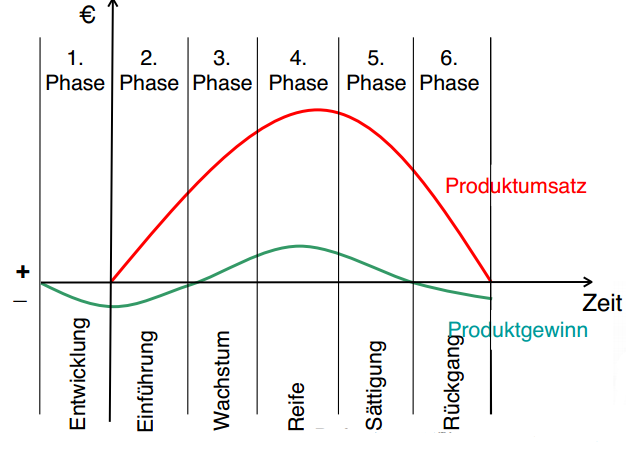
\includegraphics[scale=0.7]{Bild1_1.png}
\end{figure}


In der Graphik können wir die einzelnen Phasen ablesen, in der Entwicklung kostet das Produkt Geld, da wir Leute, Maschinen etc für die Entwicklung bezahlen müssen. Auch in der Einführungsphase beginnt der Umsatz zu steigen, allerdings kostet uns das Produkt noch Geld, da wir Geld in Werbung und oftmals Ausbesserungen stecken müssen. In der Wachstumsphase fangen wir an mit dem Produkt Geld zu verdienen, was in der Phase der Produktreife zu einem Umsatz als auch Gewinnmaximum führt. In den Phasen der Sättigung und des Rückgangs sinken der Umsatz als auch der Gewinn wieder. Zum Schluss kostet uns das Produkt wieder Geld, da wir trotz wenig bis keinen Verkäufen noch Support oder Garantieleistungen erfüllen müssen.


\subsection*{Welche Potenziale kann der Anwender von der Kopplung CAD/CAM erwarten? 
(fünf Beispiele) }


\begin{enumerate}[1)]
\item die direkte Anbindung an die Fertigung ermöglicht einen direkteren Austausch zwischen den Konstrukteuren und den Leuten an der Maschine
\item Kostensenkung: durch weniger Fehlkonstruktionen
\item Zeitersparnis: es kann schon mit CAM angefangen werden bevor CAD komplett fertig ist
\item keine Datenumwandlungen: bei verschiedenen Systemen bei CAD und CAM kann es sein, das man Daten umwandeln muss, dabei gehen oft Parameter und/oder Daten verloren
\item schnelle Ermittlung von Problemen
\end{enumerate}

\newpage

\subsection*{Was bedeuten die Kürzel und welche Tätigkeiten werden mit diesen Systemen 
unterstützt?  
Produkt entwerfen $\rightarrow$ CAD $\rightarrow$ CAE $\rightarrow$ CAP $\rightarrow$ CAM $\rightarrow$ Produkt }


\begin{description}
\item[CAD] Computer Aided Design $\Rightarrow$ Konstruieren am Rechner
\item[CAE] Computer Aided Engineering $\Rightarrow$ umfasst alle Varianten der Rechner-Unterstützung von Arbeitsprozessen in der Technik.
\item[CAP] Computer Aided Process Planning $\Rightarrow$ Werkzeugmaschinen belegen, Fertigungsmittel bereitstellen
\item[CAM] Computer Aided Manufacturing $\Rightarrow$ Spannvorrichtung festlege, Werkzeuge auswählen, Arbeitspläne erstellen, NC-Progs simulieren und bereitstellen, Produkt herstellen
\end{description}


\subsection*{Welche Informationen / Unterlagen erhalten Sie aus den Bereichen CAD, CAE, 
CAP, CAM? }

\begin{description}
\item[CAD] Zeichnungen, Stücklisten
\item[CAE] Montagepläne, Doku
\item[CAP] Maschinenbelegung, Arbeitspläne
\item[CAM] NC-Programme, Werkzeuglisten, Bestückungspläne, Korrekturen
\end{description}


\newpage

\section{NC-Programmierung}


\subsection*{Was bedeuten die Kürzel: CNC, DNC, LAN?}

\begin{description}
\item[CNC] Computerized Numerical Control
\item[DNC] Direct Numerical Control
\item[LAN] Local Area Network
\end{description}


\subsection*{Welche Informationen / Unterlagen liefert die Arbeitsplanung im Rahmen der technischen Auftragsbearbeitung?}

\begin{itemize}
\item Arbeitspläne
\item NC-Programme
\item Einrichteblätter
\item Montageblätter
\end{itemize}


\subsection*{Welche Informationen enthält ein Arbeitsplan? Erstellen Sie ein Beispiel für einen Arbeitsplan.}

Blatt, Datum, Bearbeiter, Auftragsnummer, Stückzahl, Bereich, Benennung, Zeichnungsnummer, Werkstoff, Rohform und -abmessungen, Rohgewicht, Fertigungsgew. \\
tabellarisch: AVG-Nr, Arbeitsvorgangsbeschreibung, Kostenstelle, Lohngruppe, Masch.gruppe, 
Fertigungshilfsmittel

\begin{figure}[h]
\centering
%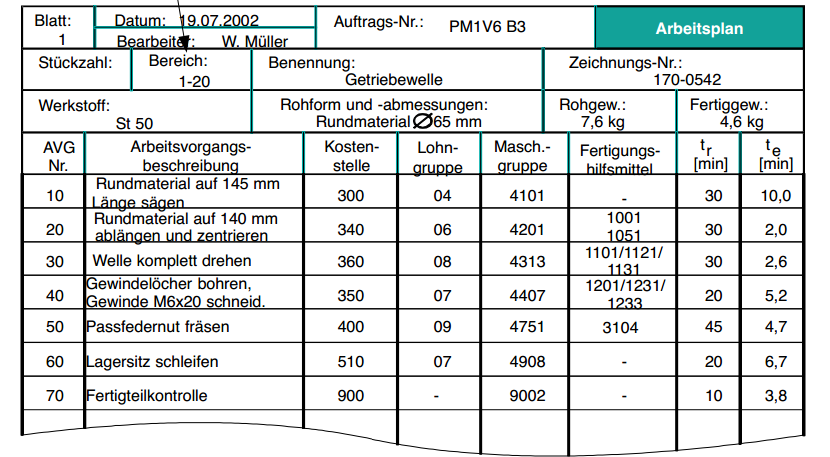
\includegraphics[scale=0.7]{Bild2_3.png}
\end{figure}


\subsection*{Welche Informationen enthält ein Einrichteblatt und welche Abteilung arbeitet mit diesen Informationen?}

Werkzeugliste, Aufspannplan, NC-Arbeitsplan, Messmittel

Abteilung:??


\subsection*{Nennen Sie drei verschiedene Möglichkeiten zur Programmierung von NC-Maschinen und beschreiben Sie in Stichworten die Unterschiede}


\begin{enumerate}[1)]
\item direkte Programmierung an der Maschine
\item direkte Programmierung an einem externen Gerät
\item Programmierung mit Hlfe einer graphischen Oberfläche und interaktiv
\item Programmierung mit Hilfe einer grafschen Oberfäche und CAD-Kopplung
\item Programmierung mit Hilfe einer grafschen Oberfäche und integriertem CAM-System
\end{enumerate}


\subsection*{Was versteht man unter „grafsch interaktiver NC-Programmierung“. Erläutern Sie drei Merkmale in Stichworten}


\begin{itemize}
\item Bearbeitungsgeometrie des Werkstücks graphisch auf dem Bildschirm
\item interaktive Eingabevorgänge $\Rightarrow$ im Dialog eingegeben, kontrolliert 
und korrigiert werden
\item Schritt für Schritt Programmierung
\item Möglichkeit zur Kopplung an CAD
\end{itemize}


\subsection*{Nennen Sie beispielhaft 5 Einsatzkriterien für grafsch interaktive Programmierung}


\begin{itemize}
\item komplizierte Teile 
\item mehr als zwei Achsen 
\item Anzahl der Maschinen 
\item Anzahl der Bearbeitungen 
\item Typenvielfalt der Maschinen 
\item Typenvielfalt der Steuerung 
\item Automatisierungsgrad der NC-Maschinen 
\item komplizierte Technologie
\item vereinheitlichte Technologie 
\item geringe Wiederholhäufigkeit 
\item CAD-Kopplung
\end{itemize}


\subsection*{Nennen Sie 3 Bezeichnungen von Schnittstellen für den Datenaustausch von CAD zu CAM-Systemen}

\begin{description}
    \item[VDAFS] Verband der Automobilindustrie – Flächenschnittstelle $\Rightarrow$ Austausch von 3D-Freiform-Kurven und –Flächendaten 
    \item[STEP] Standard for the Exchange of Product Model Data 
    \item[IGES] Initial Graphics Exchange Specification 
    \item[DXF] Drawinf Exchange Format 
    \item[STL] Standard Triangulation Language 
\end{description}


\newpage


\section{Features und Werkzeugorga}


\subsection*{Die Feature Technologie besitzt ein erhebliches Potenzial zu Beschleunigung der Produktentwicklung. Welches Problem soll mit Hilfe der \textit{Feature-Technologie} behoben werden?}

Es wird nicht mehr nur die geometrischen Elemente mit ihren festen Werten erfast, sondern auch die hinterlegten Informationen die sogenannte \glqq Semantik\grqq {} wie z.B. Funktionen und Fertigungstechnologie. \\

Ein Feature ist also eine spezifische aus Daten generierte Sichtweise auf die Produktbeschreibung, die Eigenschaftsklassen und bestimmte Phasen des Produktlebenszyklus in sich bündelt.


\subsection*{Beschreiben sie in Stichpunkten den Unterschied zwischen \glqq konventionellen\grqq {} und feature basierten CAD-Systemen.}


siehe oben.


\subsection*{Erläutern sie an einem Beispiel den Unterschied zwischen \glqq Konstriktionsfeature\grqq {} und \glqq Fertigungsfeature\grqq}


Allgemein kann man sagen, dass das Konstruktionsfeature Informationen über Teile, Material und Funktion enthält. Das Fertigungsfeature enthält Informationen wie die Bearbeitungsschritte (bohren, senken,...)

\begin{center}
\begin{figure}[h]
\begin{minipage}[hbt]{7cm}
	%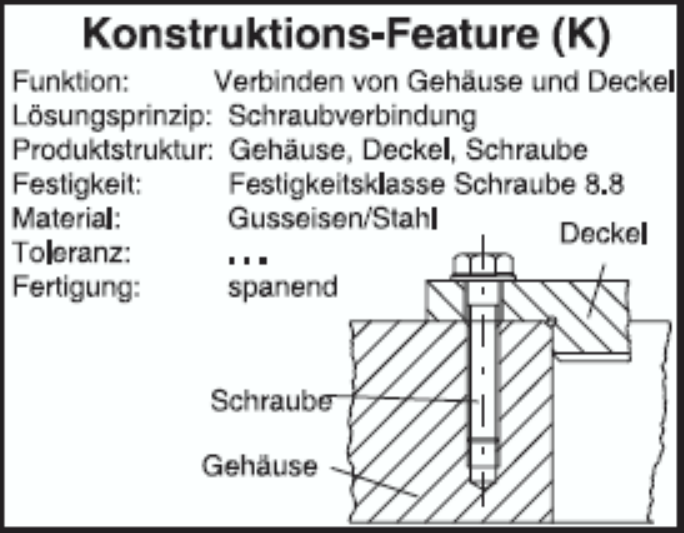
\includegraphics[width=6cm]{Bild3_3_1.png}
\end{minipage}
%
\begin{minipage}[hbt]{7cm}
	%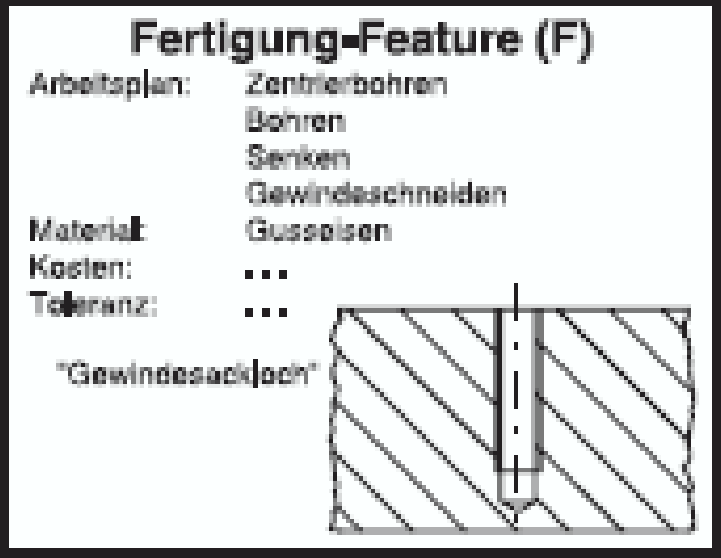
\includegraphics[width=6cm]{Bild3_3_2.png}
\end{minipage}
\end{figure}
\end{center}


\subsection*{Welche Fragen gibt es zur Featureerkennung?}

\begin{itemize}
\item Welche Maschine?
\item Welches Material?
\item Welches Werkzeug?
\item Welche Aufspannung?
\item Welche Technologie?
\item Welche Bearbeitungsreihenfolge?
\end{itemize}


\subsection*{Welche Bedeutung besitzt die Werkzeugorga im Rahmen von CAM. Erläutern sie in Stichworten.}


\begin{itemize}
\item Bessere Verfügbarkeit der Werkzeuge
\item Reduzierung der Werkzeugtypen
\item Reduzierung der Werkzeuganzahl
\item Komponenteneinsparung durh Technologiestandardisierung
\item Bessere Nutzung der Ressourcen (Wiederverwendung, Reststandzeit)
\item Vereinfachte Arbeitsplanung
\item Vereinfachte, vereinheitlichte NC-Programmierung mit Datensicherheit
\end{itemize}


\subsection*{Erläutern sie beispielhaft, warum im Zusammenhang mit dem Werkzeug eine Kollisionsbetrachtung notwendig sein kann.}


Angenommen man hat recht weit unten in einem Werkstück eine Nut, die seitlich in die Wand gefräst werden soll. Eine Kollisionsbetrachtung ist hier notwendig, da man nicht genau weiß, wie der Werkzeugkopf aufgebaut ist und wie die Maschine ihn versuchen wird in die notwendige Position zu bringen. Es könnte ja passieren, das der Operationsraum zu klein ist.


\end{document}
